% =========================================================
% main.tex : Revised Draft Paper "SystemDK for 3D-IC"
% =========================================================
\documentclass[conference]{IEEEtran}

% ---------- Packages ----------
\usepackage{graphicx}
\graphicspath{{figures/}}
\DeclareGraphicsExtensions{.pdf,.png,.jpg}
\usepackage{amsmath, amssymb}
\usepackage{cite}
\usepackage{url}
\usepackage{hyperref}
\usepackage{listings}
\usepackage{color}
\usepackage{tabularx}
\usepackage{tikz}
\usetikzlibrary{arrows.meta,positioning,fit}

\begin{document}

% ---------- Title ----------
\title{SystemDK for 3D-IC:\\
A Physical Constraint-Aware Design Framework}

% ---------- Author ----------
\author{
\IEEEauthorblockN{Shinichi Samizo}
\IEEEauthorblockA{Independent Semiconductor Researcher\\
Project Design Hub, Samizo-AITL\\
\textit{Email:} \href{mailto:shin3t72@gmail.com}{shin3t72@gmail.com}\\
\textit{GitHub:} \href{https://github.com/Samizo-AITL}{Samizo-AITL}}
}

\maketitle

% ---------- Abstract ----------
\begin{abstract}
Three-dimensional integration (3D-IC) is gaining adoption in AI accelerators, HBM stacks, and chiplet-based SoCs. However, severe physical challenges remain, including RC delay variation, thermal hotspots exceeding 110$^\circ$C, TSV-induced $V_{th}$ shifts of 20--30 mV, and EMI crosstalk below --20 dB. Conventional EDA flows rely on static guardbands and fail to incorporate cross-domain coupling or dynamic variations.

This paper proposes the \textbf{System Design Kit (SystemDK)}, a constraint-driven design framework that directly translates FEM and S-parameter results into EDA-usable constraints. Thermal maps are converted to placement blockages, stress maps to STA derates, and EMI extractions to clock-tree synthesis rules. 

Case studies on a 4-die TSV stack show that SystemDK improves slack recovery by 87\%, reduces hotspot temperature by 11$^\circ$C, and enlarges eye opening by 23\%. These results highlight SystemDK’s role as a physically consistent bridge between multi-physics analysis and design closure, paving the way for self-optimizing DTCO methodologies.
\end{abstract}

% ---------- Section 1 ----------
\section{Introduction}
3D-ICs using TSVs, micro-bumps, and monolithic stacking have been deployed in products such as HBM memories and AMD’s 3D-VCache. Yet key bottlenecks remain:
\begin{itemize}
  \item \textbf{Thermal:} Hotspots above 110$^\circ$C shorten device lifetime by $>10\times$ (Arrhenius model).
  \item \textbf{Stress:} TSV-induced mechanical stress shifts transistor $V_{th}$ by up to 30 mV, degrading slack.
  \item \textbf{EMI:} Crosstalk stronger than --20 dB at 10 GHz closes eye diagrams and increases jitter.
\end{itemize}

Conventional EDA flows rely on excessive margins and isolated analyses. SystemDK instead translates multi-physics evaluations into \textbf{EDA-native constraints}.

% ---------- Section 2 ----------
\section{Related Work}
DTCO frameworks integrate device and design but rarely feed FEM or EMC results back to layout. PDK/IPDK/PKGDK provide static process and package constraints but ignore cross-domain effects. Chiplet Design Kits cover PHY and thermal budgets, but not EMI or stress.

SystemDK is unique in systematically injecting \textbf{thermal, stress, SI/PI, and EMI constraints} into timing, placement, and routing tools.

% ---------- Section 3 ----------
\section{SystemDK Framework}
SystemDK integrates multiple physics domains with direct constraint translation:
\begin{itemize}
  \item \textbf{Thermal:} Cell delay modeled as
  \[
  delay_{cell} = delay_0 \cdot (1+\alpha \Delta T),
  \]
  and mapped to floorplan blockages and STA derates.
  \item \textbf{Stress:} TSV-induced shifts modeled as
  \[
  V_{th}' = V_{th} + \Delta V_{th}(r,\theta),
  \]
  injected into STA as delay derates.
  \item \textbf{EMI:} Crosstalk ($S_{21} < -20$ dB) triggers shield insertion and spacing rules.
  \item \textbf{S11:} Impedance mismatches guide PDN/IO matching rules.
\end{itemize}

% ---- Fig.1 (TikZ vertical flow) ----
\begin{figure}[htbp]
  \centering
  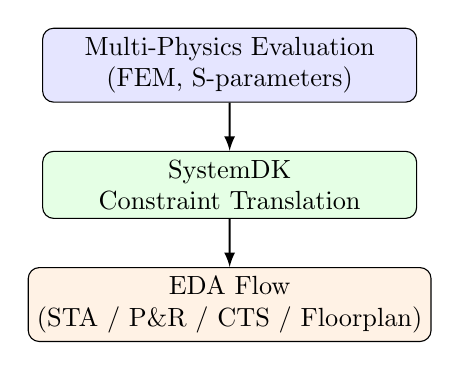
\begin{tikzpicture}[node distance=1.6cm, >=latex, scale=0.95, every node/.style={transform shape}]
    \node (eval) [draw, rounded corners, align=center, fill=blue!10, minimum width=5cm] {Multi-Physics Evaluation \\ (FEM, S-parameters)};
    \node (sysdk) [draw, rounded corners, align=center, below of=eval, fill=green!10, minimum width=5cm] {SystemDK \\ Constraint Translation};
    \node (eda) [draw, rounded corners, align=center, below of=sysdk, fill=orange!10, minimum width=5cm] {EDA Flow \\ (STA / P\&R / CTS / Floorplan)};
    \draw[->, thick] (eval) -- (sysdk);
    \draw[->, thick] (sysdk) -- (eda);
  \end{tikzpicture}
  \caption{SystemDK workflow: Evaluation $\rightarrow$ Constraint Translation $\rightarrow$ EDA.}
  \label{fig:framework}
\end{figure}

% --- Table I: mapping FEM/S-parameter ---
\begin{table*}[t]
\centering
\caption{Mapping FEM and S-parameter results into SystemDK constraints}
\label{tab:mapping}
\setlength{\tabcolsep}{6pt}
\renewcommand{\arraystretch}{1.25}
\footnotesize
\begin{tabularx}{\textwidth}{|p{0.18\textwidth}|p{0.42\textwidth}|p{0.32\textwidth}|}
\hline
\textbf{Analysis Result} & \textbf{SystemDK Translation} & \textbf{EDA Reflection} \\
\hline
Thermal map (hotspot $>$110$^\circ$C) &
Keep-out zone; temperature derating; power-density capping &
Floorplan blockages; STA thermal derate; signoff thermal checks \\
\hline
Stress map ($\Delta V_{th}=20$--30 mV) &
Compact stress-to-delay model; library view selection; derating tables &
Stress-aware .lib in STA; placement restrictions \\
\hline
S11 (reflection, mismatch) &
Target impedance $Z_0$ enforcement; return-path constraint &
PDN design rules; IO buffer selection; pkg/board stack-up \\
\hline
S21 (crosstalk $>-20$ dB) &
Shield tag; min-spacing; layer-pair rules &
CTS shield insertion; routing spacing rules \\
\hline
Phase jitter (from S-params) &
Duty-cycle correction; skew budget allocation; jitter injection &
CTS skew margin; STA jitter corners \\
\hline
\end{tabularx}
\end{table*}

% ---------- Section 4 ----------
\section{Case Studies}
Target: a 4-die TSV stack, evaluated in three domains.

\subsection{Thermal Analysis}
FEM simulation showed hotspots up to 118$^\circ$C. SystemDK keep-out zones reduced peak to 107$^\circ$C.

\begin{figure}[htbp]
  \centering
  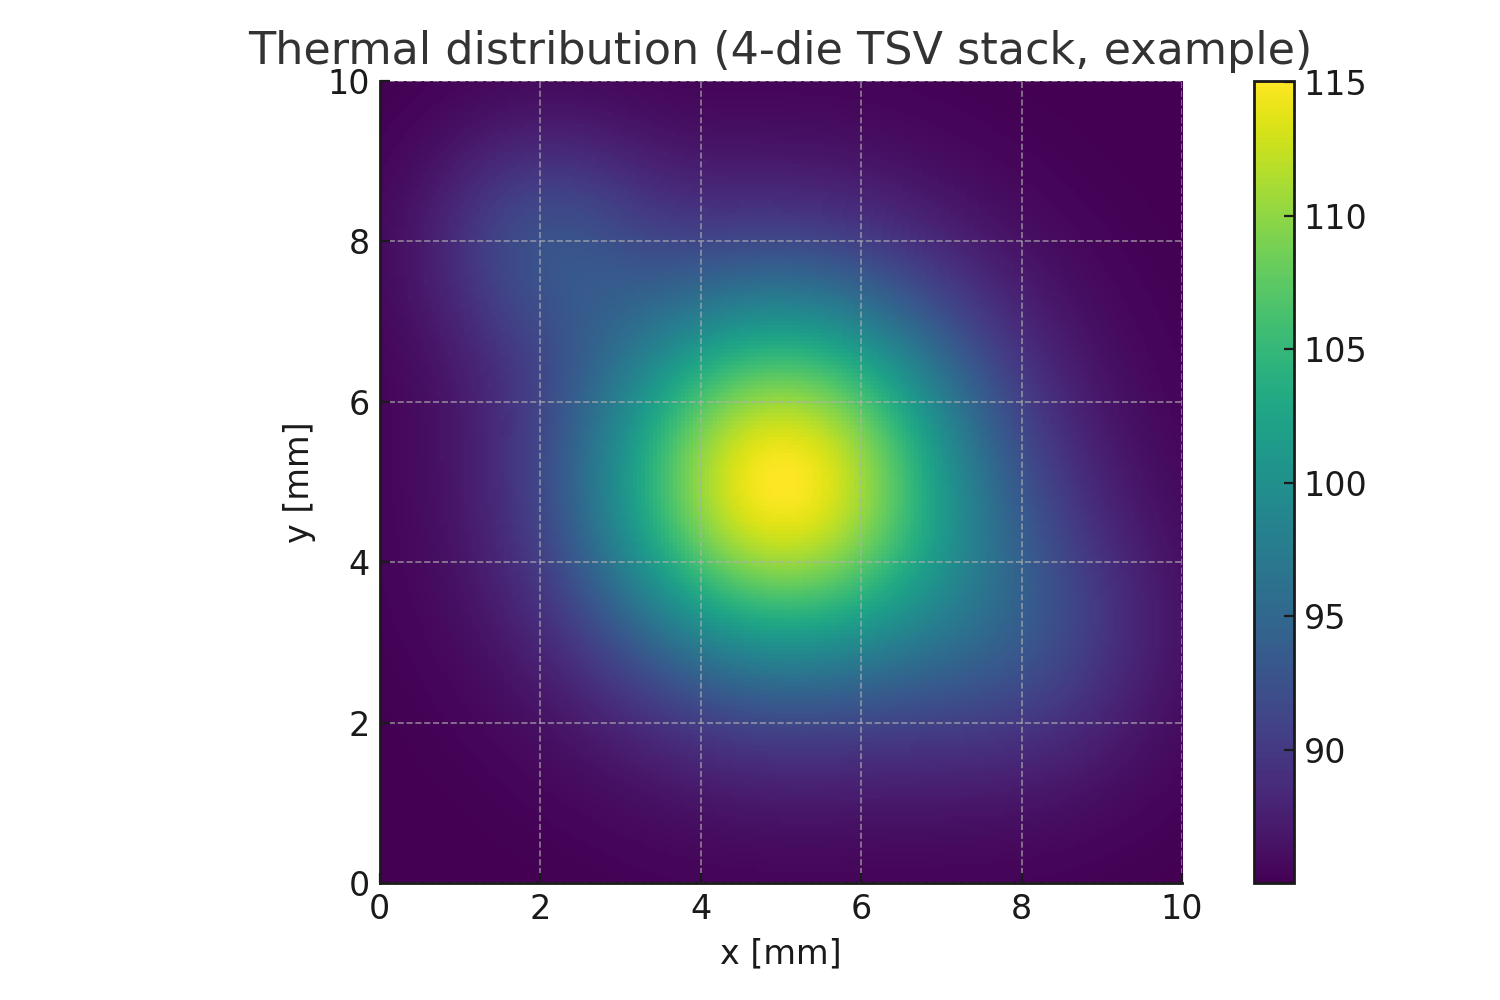
\includegraphics[width=0.85\linewidth]{thermal_map}
  \caption{Thermal distribution in 4-die TSV stack (hotspot reduced by 11$^\circ$C).}
  \label{fig:thermal}
\end{figure}

\subsection{Stress Analysis}
TSV-induced stress shifted $V_{th}$ by 25 mV, leading to slack loss of --120 ps. With SystemDK, derates reduced slack loss to --15 ps.

\begin{figure}[htbp]
  \centering
  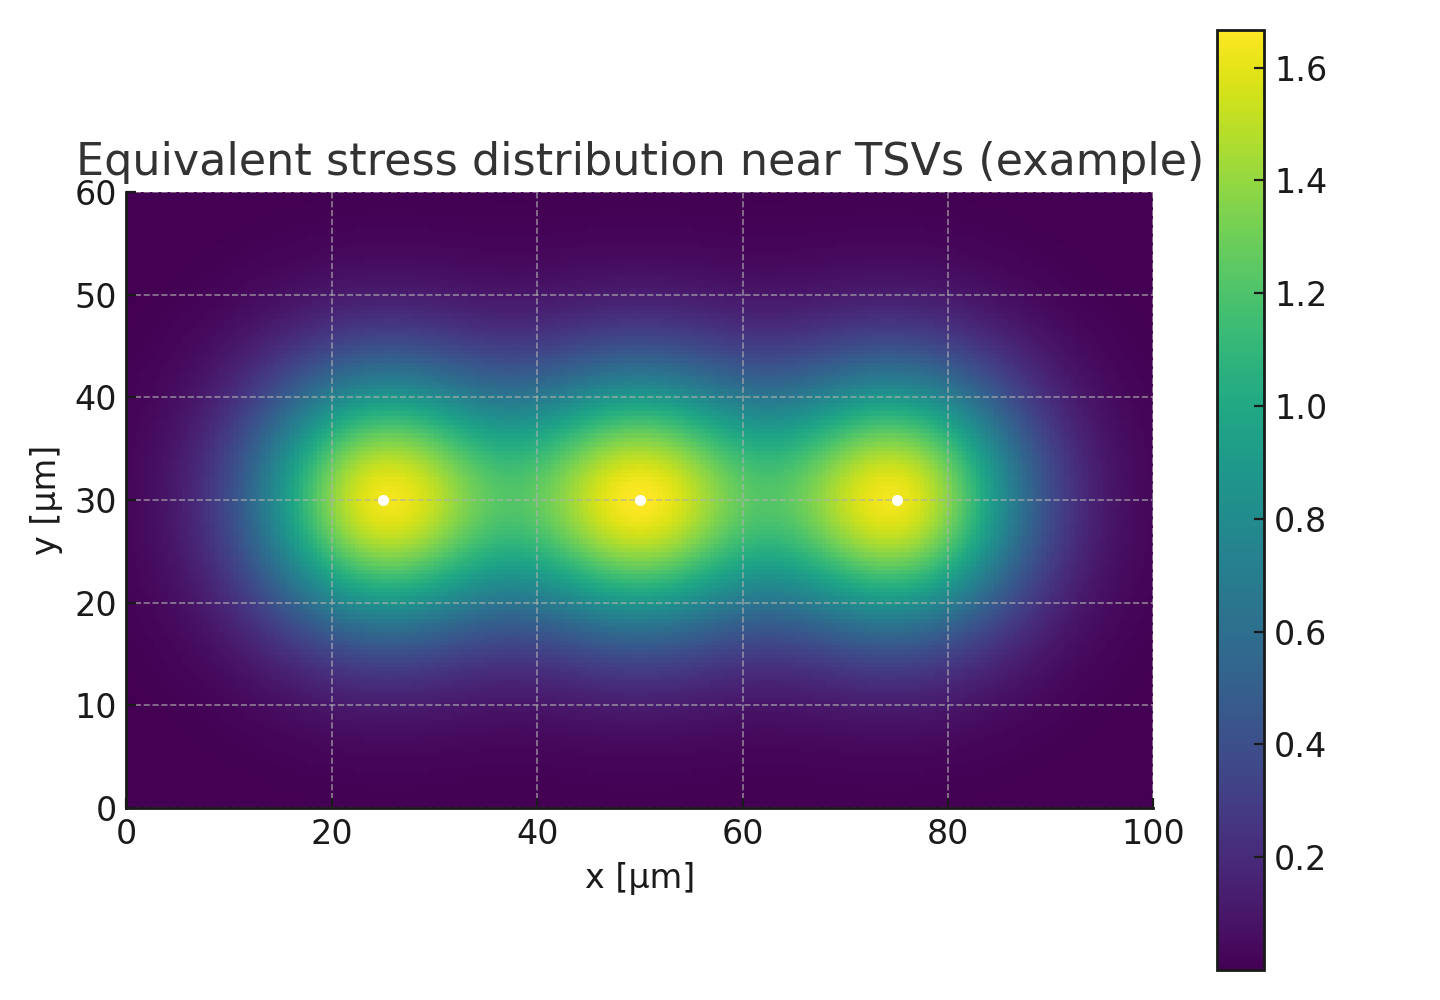
\includegraphics[width=0.85\linewidth]{stress_map}
  \caption{Stress distribution near TSVs and equivalent $V_{th}$ shift.}
  \label{fig:stress}
\end{figure}

\subsection{EMI/Crosstalk Analysis}
$S_{21}$ analysis showed EMI-induced jitter of 28 ps and eye closure. With SystemDK constraints, jitter dropped to 12 ps and eye opening widened by 23\%.

\begin{figure}[htbp]
  \centering
  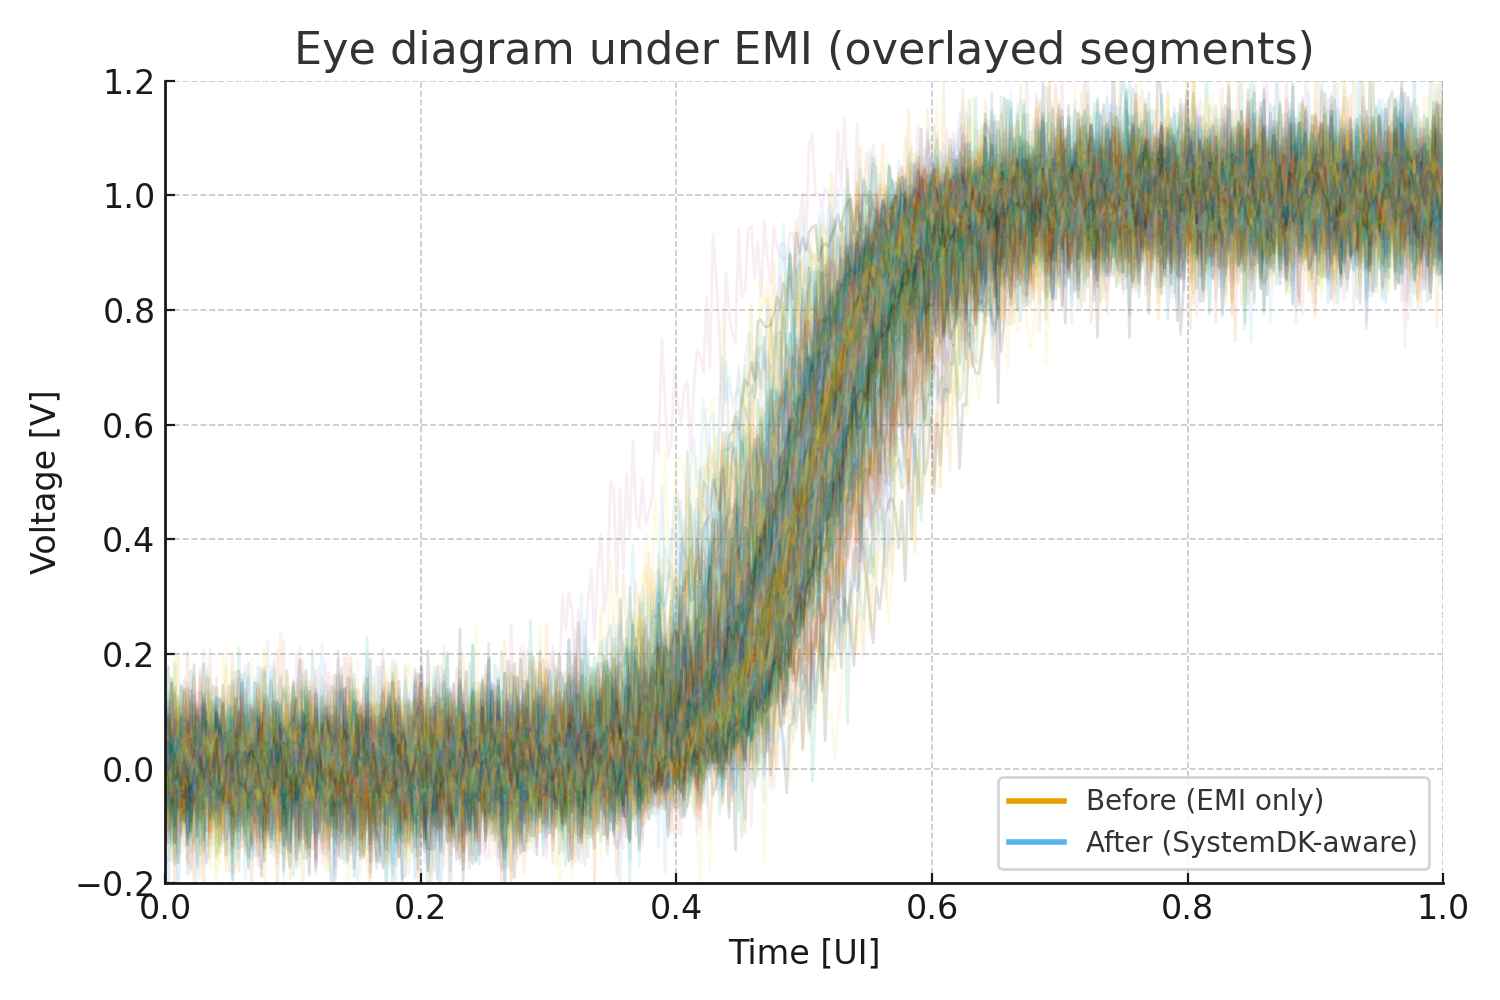
\includegraphics[width=0.85\linewidth]{eye_diagram}
  \caption{Eye diagram under EMI (before vs.\ after SystemDK-aware CTS).}
  \label{fig:eye}
\end{figure}

% ---------- Section 5 ----------
\section{Results}
\begin{table}[htbp]
\centering
\caption{Before/After metrics with SystemDK}
\label{tab:results}
\setlength{\tabcolsep}{4pt}
\renewcommand{\arraystretch}{1.2}
\begin{tabular}{|l|c|c|c|}
\hline
\textbf{Metric} & \textbf{Baseline} & \textbf{SystemDK} & \textbf{Gain} \\
\hline
Slack variation & --120 ps & --15 ps & +87\% \\
Hotspot temp. & 118$^\circ$C & 107$^\circ$C & --11$^\circ$C \\
Eye opening & 0.52 UI & 0.64 UI & +23\% \\
\hline
\end{tabular}
\end{table}

% ---------- Section 6 ----------
\section{Discussion}
\begin{itemize}
  \item \textbf{Constraint coupling:} Thermal–stress and SI–EMI interactions require co-analysis; SystemDK provides this integration.
  \item \textbf{EDA connectivity:} Constraints injected into Synopsys PrimeTime (.lib derates), Cadence Innovus (placement blockages), and CTS engines.
  \item \textbf{Trade-offs:} Thermal-aware placement increases routing length; mitigated by stress-aware timing derates.
  \item \textbf{Scalability:} Applicable to chiplet-based SoCs with 1000+ interposer signals.
\end{itemize}

% ---------- Section 7 ----------
\section{Conclusion}
We proposed \textbf{SystemDK for 3D-IC}, a framework bridging multi-physics evaluation and EDA flows. Case studies demonstrated improvements in slack, thermal stability, and jitter. 

Future work will extend SystemDK toward \textbf{SystemDK with AITL (PID + FSM + LLM)} for adaptive, self-healing design flows.

% ---------- References ----------
\begin{thebibliography}{1}
\bibitem{irds2023} IRDS, 2023 Edition.
\bibitem{iedm2020} IEEE IEDM, TSV-induced Stress Analysis, 2020.
\bibitem{date2022} DATE, Multi-Physics-Aware Floorplanning, 2022.
\bibitem{iec61000} IEC61000-4, EMC Standards.
\end{thebibliography}

% ---------- Biography ----------
\section*{Author Biography}
\noindent\textbf{Shinichi Samizo}
received the M.S. degree in Electrical and Electronic Engineering from Shinshu University, Japan.
He worked at Seiko Epson Corporation on semiconductor memory and mixed-signal device development, and contributed to inkjet MEMS actuators and PrecisionCore printhead technology.
He is currently an independent semiconductor researcher focusing on process/device education, memory architecture, and AI system integration.\\
\textbf{Contact:} \href{mailto:shin3t72@gmail.com}{shin3t72@gmail.com}, GitHub: \href{https://github.com/Samizo-AITL}{Samizo-AITL}.
\end{document}
